\chapter{Crypto.Symmetric.KDF}
Key Derivation Functions (in the following “KDFs”) are a mean for deriving a secret key with specific properties from a secret value, often a string or a byte sequence, and the salt, additional information. The KDFs have different properties regarding CPU and memory usage, fitting a various set of application.
\section{API}
\subsubsection*{Types}
\begin{lstlisting}{}
   type return_type is private;
   type KDF_Scheme is limited interface;
\end{lstlisting}
The type of the \texttt{return\_type} sets the return type, mostly Bytes. The \texttt{KDF\_Scheme} contains required internal information of the respective KDF.
\subsection*{Procedures}
\begin{lstlisting}{}
   procedure Derive(This	: in out KDF_Scheme'Class;
                    Salt	: in 	String;
                    Password	: in	String;
                    Key		: out	Return_Type);

   procedure Derive(This	: in out KDF_Scheme;
                    Salt	: in 	Bytes;
                    Password	: in	Bytes;
                    Key		: out	Return_Type) is abstract;

   procedure Initialize(This	: out KDF_Scheme;
                        Key_Length : in Natural) is abstract;

\end{lstlisting}
The API provides a function for initialization as well as two flavors of key derivation. More Variation may be found in the specific KDFs. 

\section{PBKDF2}

\begin{figure}[ht!]
\centering
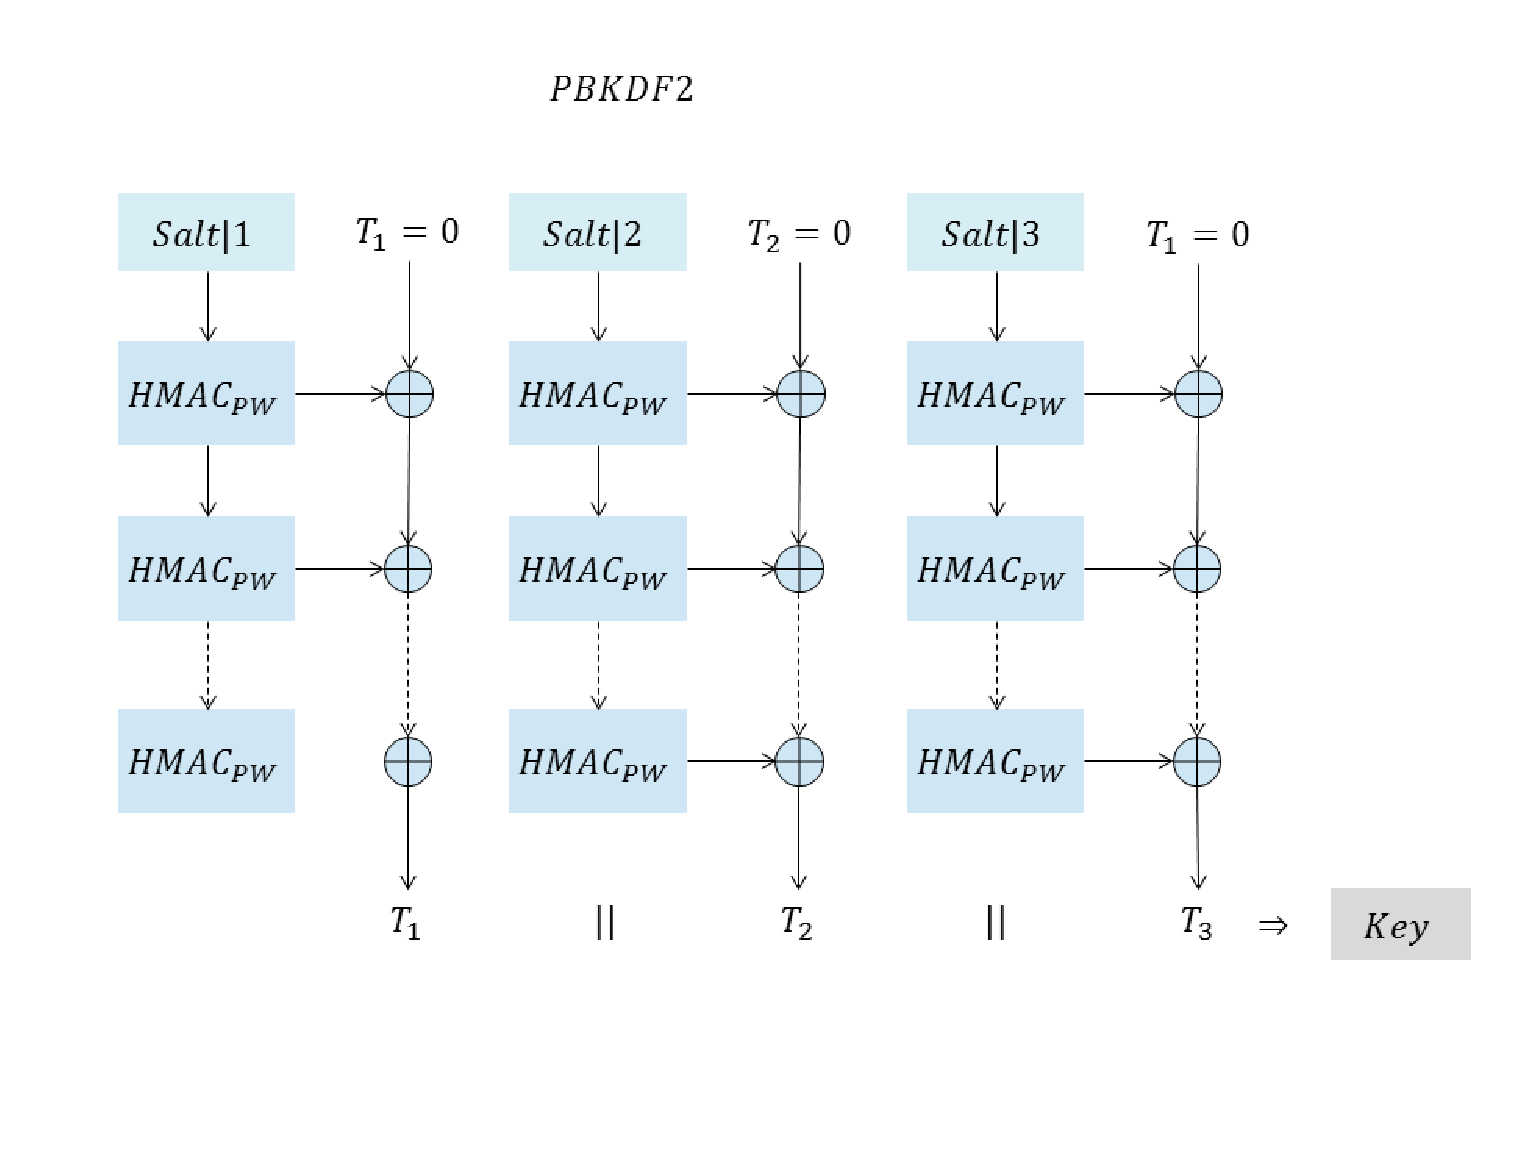
\includegraphics[width=150mm]{./images/PBKDF2}
\caption{The structure of PBKDF2}
\end{figure}

Password Based Key Derivation Function 2 is a KDF, which uses HMAC with SHA1 as a pseudo-random function, which is applied multiple times. It builds the keys from multiple parts depending on the size of the used hash functions output and the desired key size. 
\subsubsection*{Types}
\begin{lstlisting}{}
package KDF is new Crypto.Symmetric.KDF(Return_Type        => Bytes,
                                           H                  => Hmac_Package.H);
   type PBKDF2_KDF is new KDF.KDF_Scheme with private;

\end{lstlisting}
PBKDF2 takes salt and password as input, and has the parameters key size and round count .

\subsection*{Functions}
\begin{lstlisting}{}
   overriding
   procedure Derive(This	: in out PBKDF2_KDF;
                    Salt	: in 	Bytes;
                    Password	: in	Bytes;
                    Key		: out	Bytes);
										
	 overriding
   procedure Initialize(This	: out PBKDF2_KDF;
                        Key_Length: in Natural);

   procedure Initialize(This		: out PBKDF2_KDF;
                        Key_Length	: in Natural;
                        Round_Count	: in Natural);

\end{lstlisting}
\begin{itemize}
	\item The function \texttt{Derive()} derives a Key from the Input
	\item The function \texttt{Initialize()} sets the \texttt{Key\_Length} or the \texttt{Key\_Length} and the \texttt{Round\_Count};
\end{itemize}
The API provides a function for derivation as well as two flavors of initialization, one with key length and one with key length and round count.

\section{Sha512crypt}

\begin{figure}[ht!]
\centering
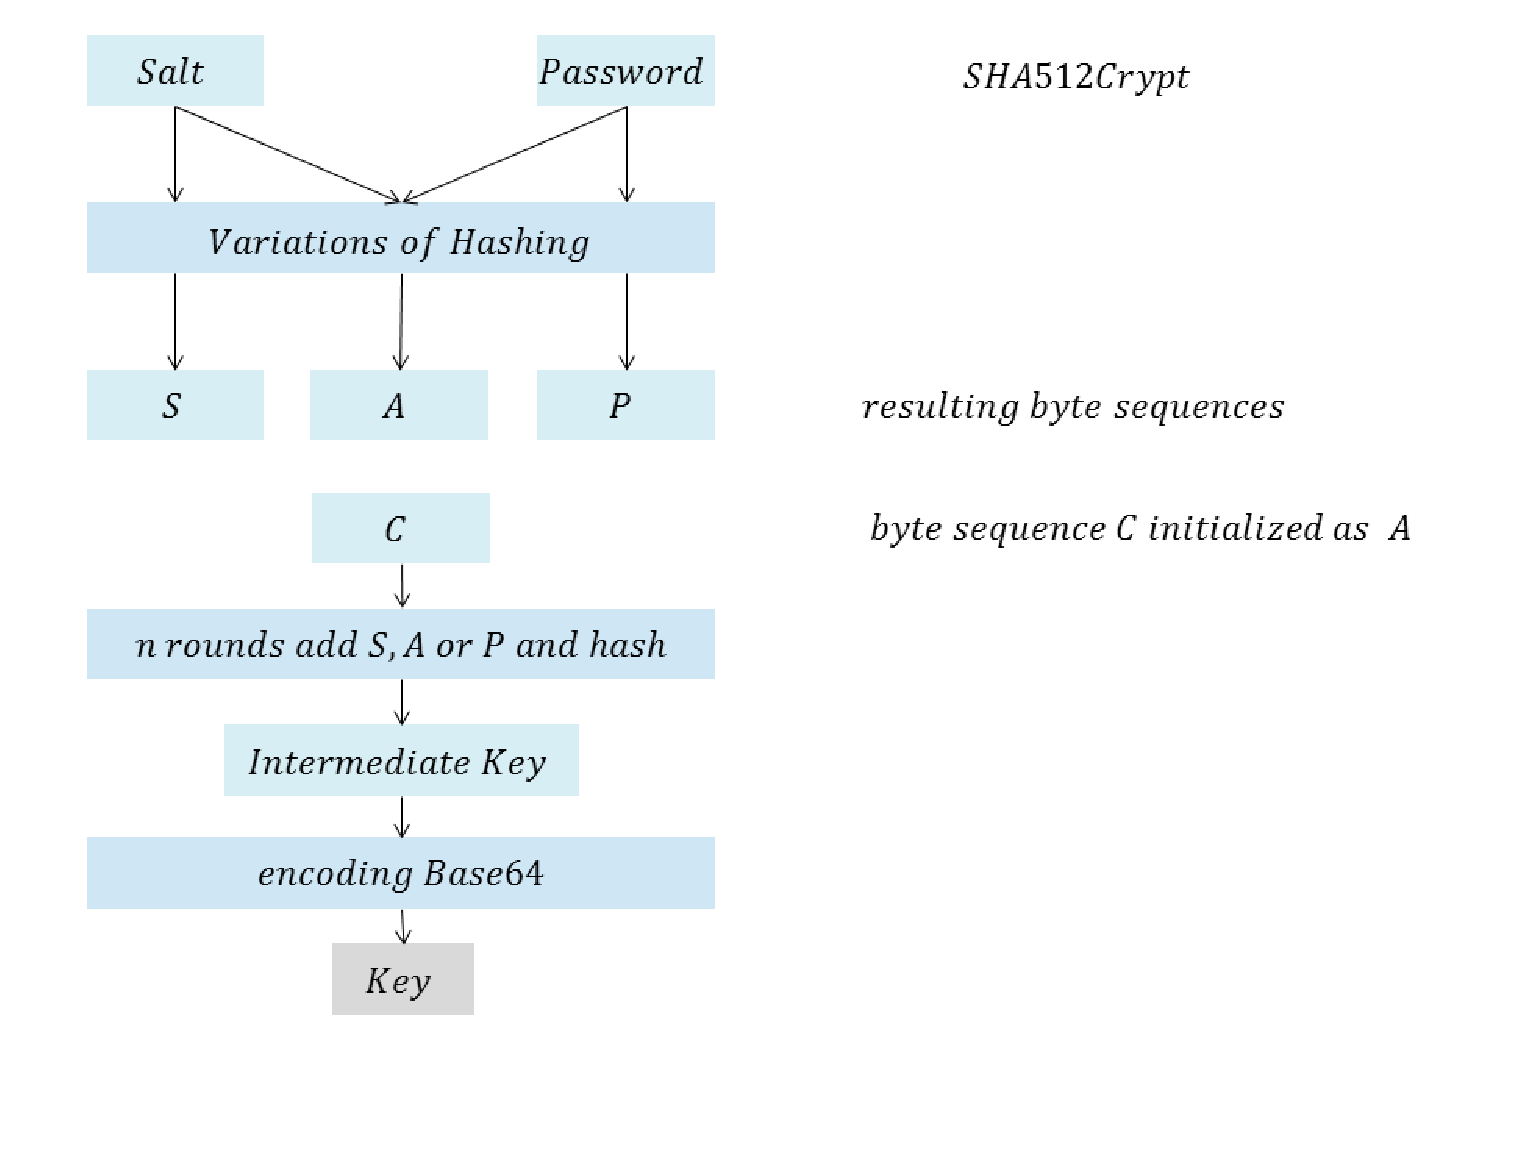
\includegraphics[width=150mm]{./images/SHA512Crypt}
\caption{The structure of SHA512Crypt}
\end{figure}

Sha512Crypt derives a key of a fixed size(86) from a salt and a password string. Those are \texttt{Round\Count} rounds long in variations hashed, mixed and concatenated and finally encoded base64.
\subsubsection*{Types}
\begin{lstlisting}{}
   package KDF is new Crypto.Symmetric.KDF(Return_Type        => Base64_String,
                                           H                  => Crypto.Symmetric.Hashfunction_SHA512);


\end{lstlisting}
Subtype \texttt{S5C\_String} is the fixed-length output string, The round count, a natural, is defined by the \texttt{Round\_Count}. \texttt{SHA512Crypt\_KDF} implements the \texttt{KDF\_Scheme}, containing only the \texttt{security\_parameter}. 

\subsection*{Functions}
\begin{lstlisting}{}
   overriding
   procedure Derive(This	: in out SHA512Crypt_KDF;
                    Salt	: in 	Bytes;
                    Password	: in	Bytes;
                    Key		: out	Base64_String);
   overriding
   procedure Initialize(This	: out SHA512Crypt_KDF;
                        Key_Length: in Natural);

   procedure Initialize(This		: out SHA512Crypt_KDF;
                        Key_Length	: in Natural;
                        Round_Count	: in Natural);


\end{lstlisting}
\begin{itemize}
	\item The function \texttt{Derive()} derives a Key from the Input, overriding the \texttt{KDF} function.
	\item The functions \texttt{Initialize()}, overriding \texttt{Initialize()} from the KDF, set the \texttt{Round\_Count} or \texttt{Round\_Count} and \texttt{Key\_Length}.
\end{itemize}


\section{SCrypt}
SCrypt relies on a group of nested functions for deriving a Key from a Salt and a Password Input. It uses the additional parameters Cost Parameter and Parallelization Parameter in the Computation for adjusting the CPU and Memory costs.
\subsubsection*{Types}
\begin{lstlisting}{}
package KDF is new Crypto.Symmetric.KDF(Return_Type        => W_Block512,
                                           H                  => Crypto.Symmetric.Hashfunction_SHA512);

type Scrypt_KDF is new KDF.KDF_Scheme with private;

\end{lstlisting}

\begin{figure}[ht!]
\centering
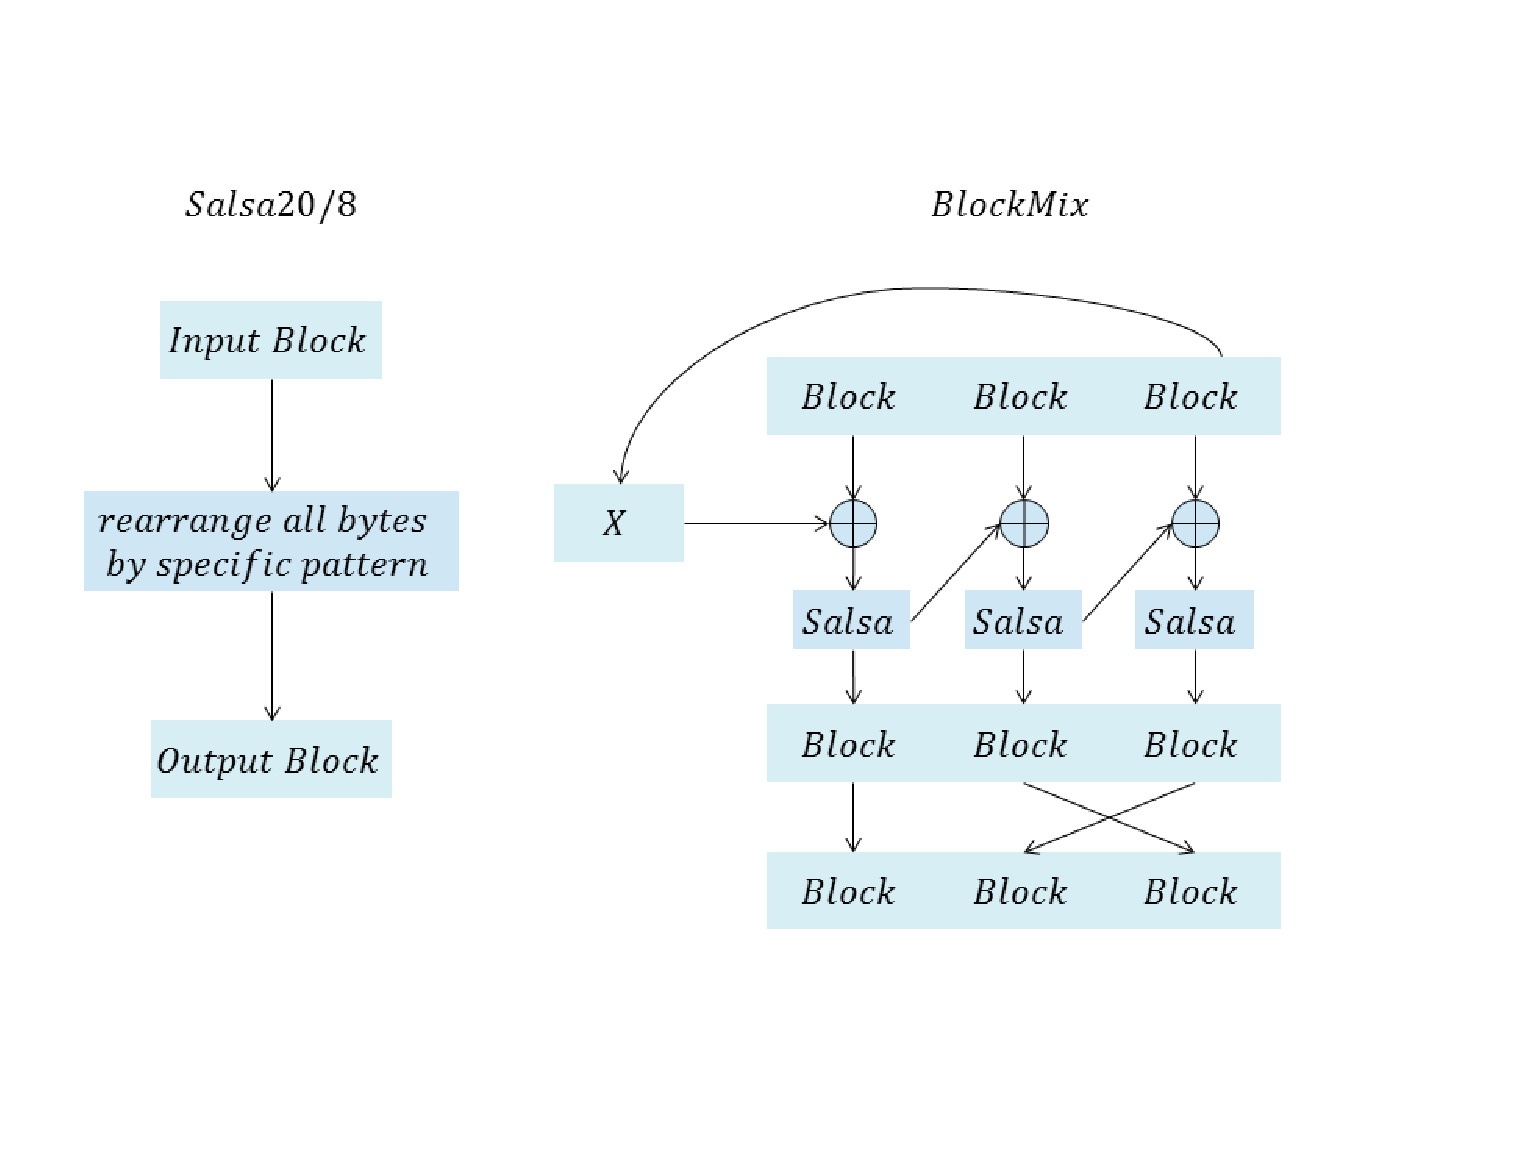
\includegraphics[width=150mm]{./images/Scrypta}
\caption{The structure of SCrypt, part 1}
\end{figure}

\begin{figure}[ht!]
\centering
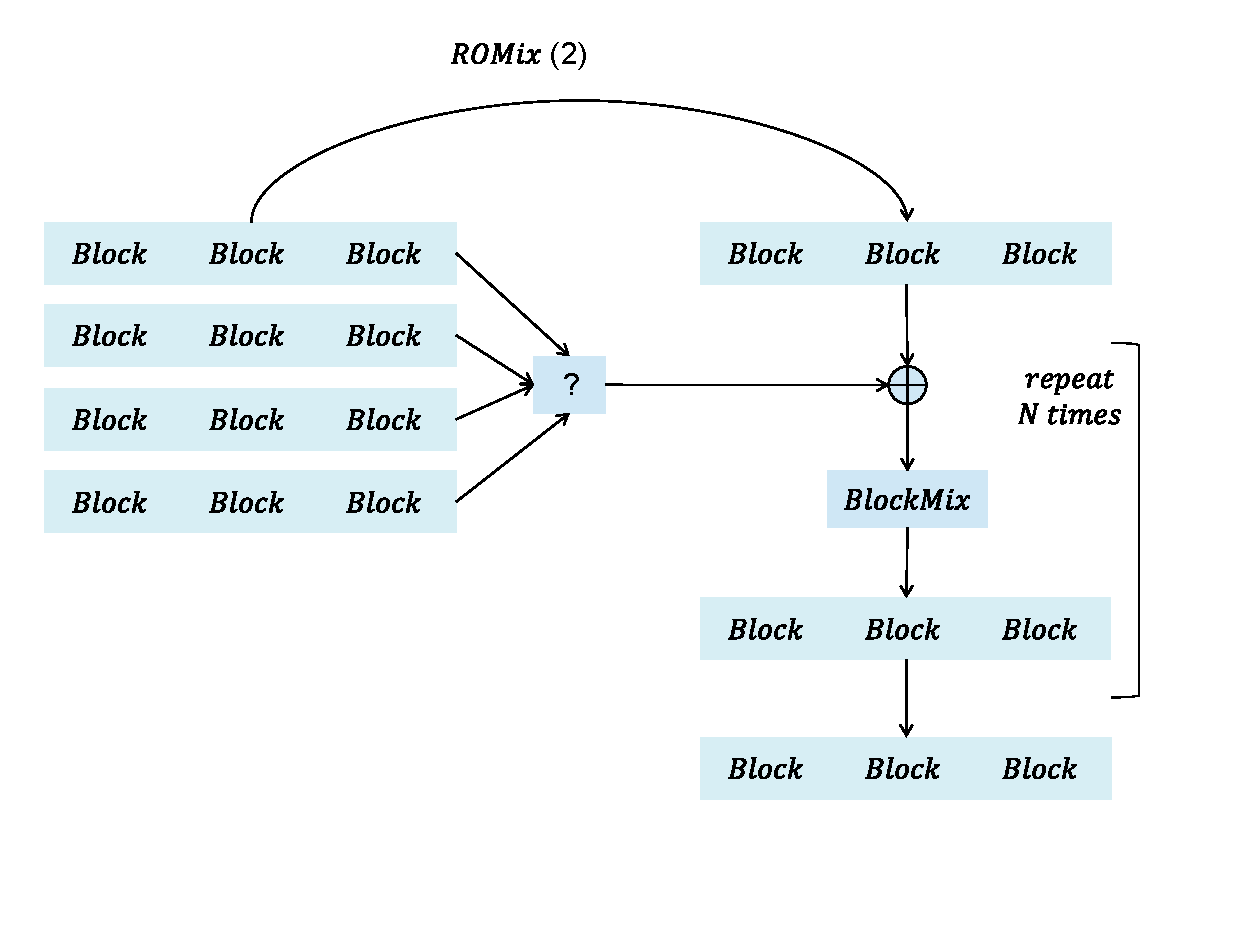
\includegraphics[width=150mm]{./images/Scryptb}
\caption{The structure of SCrypt, part 2}
\end{figure}

\begin{figure}[ht!]
\centering
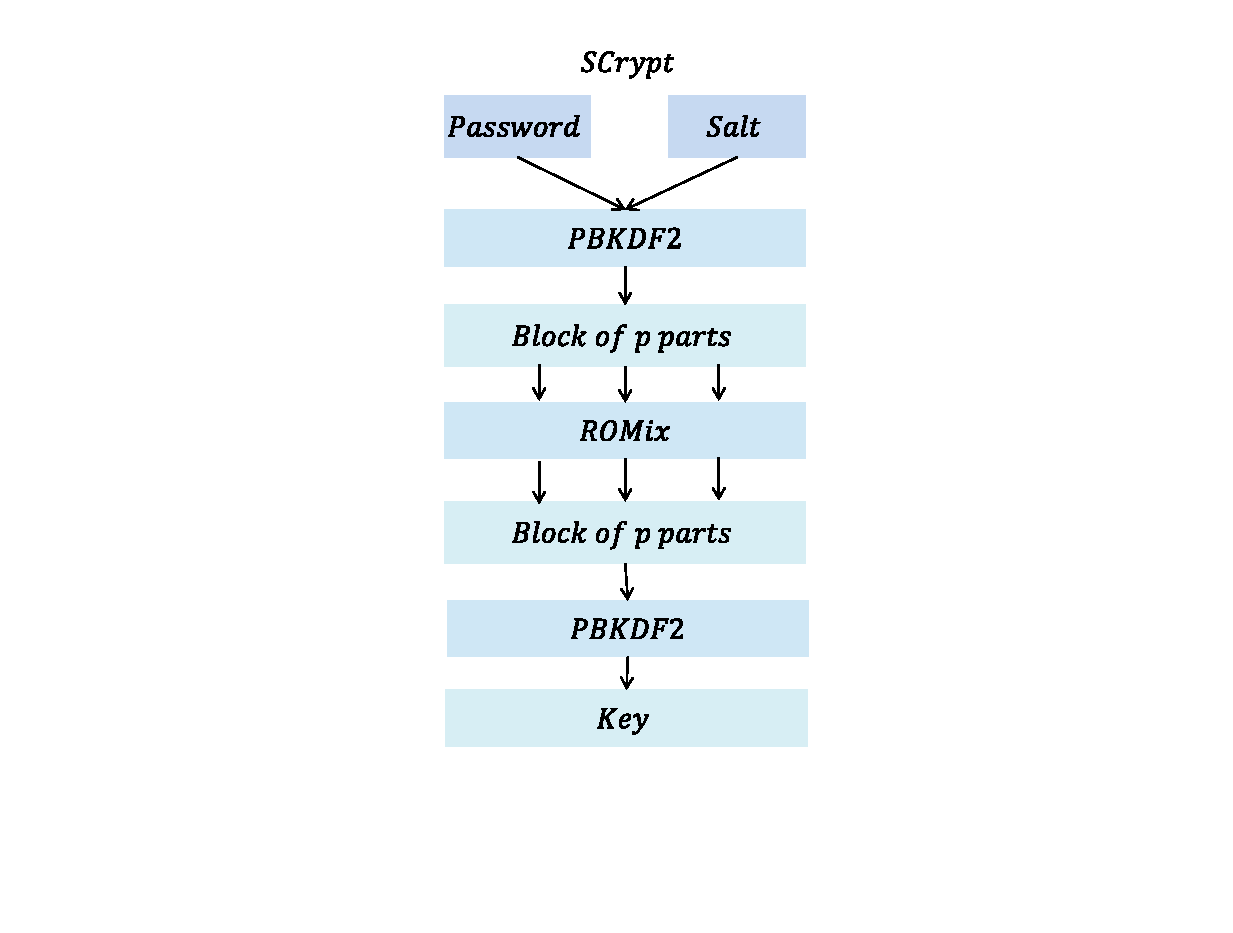
\includegraphics[width=150mm]{./images/Scryptc}
\caption{The structure of SCrypt, part 3}
\end{figure}

Scrypt can return arbitrary key lengthes. One Initialize is provided only with the \texttt{Key\_Size}, one with all Parameters of SCrypt.

\subsection*{Functions}
\begin{lstlisting}{}
   overriding
   procedure Derive(This	: in out Scrypt_KDF;
                    Salt	: in 	Bytes;
                    Password	: in	Bytes;
                    Key		: out	W_Block512);
   overriding
   procedure Initialize(This	: out Scrypt_KDF;
                       Key_Length: in Natural);


   procedure Initialize (This	: out Scrypt_KDF;
                         r		: in 	Natural;
                         N		: in 	Natural;
                         p		: in	Natural;
                         dkLen	: in	Natural);

\end{lstlisting}
\begin{itemize}
	\item The function \texttt{Derive()} derive a Key from the Input, overriding the KDF functions.
	\item The functions \texttt{Initialize()} offer setting of all variables of scrypt.
	\item The procedure \texttt{scrypt()} offers the complete scrypt implementation, enabling the user to set all parameters provided by the algorithm.
\end{itemize}

